\documentclass[12pt]{article}
\usepackage[T1]{fontenc}
\usepackage[utf8]{inputenc}
\usepackage{lmodern}
\usepackage[margin=1in]{geometry}
\usepackage{amsmath,amssymb}
\usepackage{graphicx}
\usepackage{booktabs,tabularx,array}
\usepackage{setspace}
\usepackage[labelfont=bf,font=small]{caption}
\usepackage[hidelinks]{hyperref}
\usepackage{float}
\setstretch{1.15}
\setlength{\parskip}{4pt}
\title{STAR: A Sensitivity-Analysis Framework for Off-Policy Evaluation When Mobile Health Rewards Are Missing Not at Random}
\author{Selorm Buaka\\PhD Student, Applied Statistics and Research Methods\\University of Northern Colorado}
\date{\today}
\begin{document}
\maketitle
\begin{abstract}

Micro-randomized trials (MRTs) are the main source of data for evaluating mobile health decision rules offline, but their wearable outcomes go missing when people stop wearing the device. If non-wear is linked to the steps a person would have taken, standard off-policy evaluation (OPE) is biased, and the observed data cannot reveal how large that bias is. We propose STAR, a sensitivity-analysis framework for OPE when rewards are missing intermittently, in spells, and possibly not at random. An exponential-tilt parameter $\delta$ sets the assumed departure from missing at random, and policy values are estimated across a range of $\delta$ with two estimators: STAR-EM, a joint model of the reward and its missingness fitted by a semiparametric EM algorithm, and STAR-DR, a tilted doubly robust estimator. In a plasmode simulation built from HeartSteps (7,300 simulated trials, eight scenarios), both estimators removed most of the bias when $\delta$ was set correctly, while standard methods were off by up to 250 steps per day when missingness depended on the intervention. STAR-DR was the only correction that stayed close to unbiased when missingness ran through a hidden activity state, and it was about eight times cheaper to compute. In HeartSteps itself, no policy contrast differed from zero under missing at random or anywhere on the tilt grid from $-$1.5 to 1.5, and worst-case bounds were too wide to rule out large effects in either direction. We recommend STAR-DR as the default, with STAR-EM as a check.

\end{abstract}

\section{Introduction}

Just-in-time adaptive interventions decide, at each of many decision points, whether to send a prompt such as a suggestion to go for a walk. Micro-randomized trials (MRTs) randomize that prompt with a known probability at every decision, which makes them the natural data source for judging a new decision rule before it is deployed (Klasnja et al., 2019). In reinforcement learning terms this is off-policy evaluation (OPE): we estimate the value of a target policy using data collected under the trial's behaviour policy. Because the behaviour policy is known, importance sampling and doubly robust estimators are unbiased when every reward is recorded (Jiang \& Li, 2016).

Such interventions are built from a small set of components: decision points, the information available at each one (tailoring variables), the intervention options, and decision rules that map the information to an option (Nahum-Shani et al., 2018). Most statistical work on MRT data has focused on the first-order question of whether a prompt works at all, through causal excursion effects that compare sending with not sending at a decision point, possibly moderated by context (Boruvka et al., 2018). Those effects are averaged over the trial's own randomization. A designer choosing among decision rules needs something different: the value of each rule if it were followed for a whole day, including how earlier prompts change later availability and behaviour. That is a sequential, policy-level question, and it is the one OPE answers.

With wearable outcomes, rewards are often not recorded. In HeartSteps V1 the 30-minute step count after a decision is missing for 9.4\% of decisions, and the gaps come in runs: after a missing reward the next one is missing 66.8\% of the time, against 3.7\% after an observed one. Device non-wear is a common source of missing outcomes in MRTs (Zhang et al., 2025). People may well take the tracker off on inactive or difficult days. If so, the rewards are missing not at random (MNAR), and an analysis that assumes missing at random (MAR) will overstate how active people were and may favour the wrong policy.

The data cannot settle how far from MAR the missingness is. Any MNAR analysis therefore rests on an assumption that the observed data cannot check, and the honest output is a sensitivity analysis: how the conclusion changes as the assumed departure from MAR grows (Scharfstein et al., 1999). Existing OPE methods for MNAR rewards take a different route: they identify the missing rewards through a shadow variable, an assumption that also cannot be checked, and MRT-specific methods assume MAR (Section 2).

This paper makes three contributions:

\begin{enumerate}

\item \textbf{A sensitivity-analysis framework for OPE with MNAR rewards.} STAR handles rewards missing intermittently and in spells. One parameter $\delta$ indexes the departure from MAR, and it may differ on decisions where a prompt was sent. The framework needs no shadow variable and no reward distribution.

\item \textbf{Two estimators, compared head to head.} STAR-EM models the reward and its missingness jointly, including a possible hidden activity state, and fits the model by EM. STAR-DR corrects each reward through a tilted, doubly robust pseudo-reward. A plasmode simulation built from HeartSteps shows when each one works and what each costs to compute.

\item \textbf{An applied analysis.} A tipping-point analysis of four HeartSteps notification policies, with worst-case bounds that assume nothing about the missingness.

\end{enumerate}

The rest of the paper is organized as follows. Section 2 reviews related work. Section 3 sets out the data structure and the sensitivity assumption. Section 4 describes the two estimators and how intervals and bounds are computed. Section 5 reports the simulation study, Section 6 the HeartSteps analysis, Section 7 discusses recommendations and limitations, and Section 8 concludes.

\section{Related work}

STAR draws on five lines of work: off-policy evaluation, missing outcomes in MRTs, OPE with nonignorable missing rewards, sensitivity analysis for MNAR data, and joint models fitted by EM. Table 1 summarizes the closest of them.

\textbf{Off-policy evaluation.} Importance sampling estimates the value of a target policy by reweighting observed rewards by the ratio of target to behaviour action probabilities. Per-decision importance sampling applies only the ratios up to the current decision, which lowers variance without adding bias (Precup et al., 2000). Doubly robust estimators add a model of the value function and use the importance ratios to correct its errors, so they remain unbiased when the behaviour policy is known and are less variable when the value model is good (Jiang \& Li, 2016). In observational data the behaviour policy has to be estimated, and that is usually the main source of bias. In an MRT it is known by design, so the remaining problem is the reward itself.

\textbf{Missing outcomes in MRTs.} Zhang et al. (2025) review how missing outcomes are handled in MRTs: complete-case analysis, multiple imputation, and missing-data indicators. They describe device non-wear as a common cause, but the methods they review assume MAR and none evaluates a whole decision policy. Yu and Qian (2024) give a doubly robust estimator of causal excursion effects when longitudinal outcomes are missing, again under MAR. An excursion effect is the average effect of sending versus not sending a prompt at one decision, not the value of a policy followed over a day, so neither line of work answers the OPE question when missingness is informative.

\textbf{OPE with nonignorable missing rewards.} Two recent papers address MNAR rewards in OPE directly. Wang et al. (2025) study monotone dropout, where a trajectory stops being observed and never resumes, and identify the missing rewards through a shadow variable, a variable related to the reward but not to missingness once the reward is known. Their estimator includes a semiparametric exponential tilt and inverse-probability weighting. Wei et al. (2026) use the next state as the shadow variable inside fitted-Q evaluation and test their method on synthetic missingness. Both approaches recover the policy value without a sensitivity parameter, but only if the shadow-variable condition holds, and that condition cannot be checked from the data. In wearable studies the next state is often missing in the same non-wear spell as the reward, which makes it a weak shadow variable. STAR makes the opposite trade: it gives up point identification and reports how conclusions change across a range of assumptions.

\textbf{Sensitivity analysis for MNAR data.} Scharfstein et al. (1999) introduced the exponential-tilt selection model for dropout in clinical trials. One parameter links the distribution of missing outcomes to that of observed outcomes with the same history, and its value is varied rather than estimated. The tilt is easy to interpret: a negative value means missing outcomes are lower than observed ones. At the other extreme, worst-case bounds (Horowitz \& Manski, 2000) replace each missing outcome by the smallest or largest possible value and so assume nothing about the missingness. STAR uses both: the tilt for the main analysis and the bounds as a reference.

\textbf{Joint models fitted by EM.} Shared-parameter models link an outcome and its missingness through a common latent variable, so the two are dependent even when neither depends on the other directly (Follmann \& Wu, 1995). Hidden Markov models extend this to a latent state that changes over time, and with enough repeated measurements per person their structure is identified even when the emission distributions are nonparametric (Gassiat et al., 2016). Such models are fitted by EM (Dempster et al., 1977), which handles the unobserved rewards and states as missing data. STAR-EM brings this machinery into OPE for the first time, as far as we know.

\begin{table}[!htbp]\centering\small
\caption{Closest existing work and what STAR adds.}
\begin{tabularx}{\textwidth}{>{\raggedright\arraybackslash}p{0.22\textwidth}XX}
\toprule
\textbf{Work} & \textbf{What it covers} & \textbf{What it leaves open} \\
\midrule
Wang et al. (2025) & OPE with monotone dropout; MNAR identified through a shadow variable; tilted IPW estimator & Intermittent missingness in spells; settings without a credible shadow variable \\
Wei et al. (2026) & OPE with MNAR rewards; next state as shadow variable inside fitted-Q evaluation & Real missingness; dependence between successive missing rewards; an untestable identifying condition \\
Yu \& Qian (2024) & Missing outcomes in MRTs under MAR; causal excursion effects & MNAR; values of whole policies \\
Zhang et al. (2025) & Review of missing data in MRTs & No MNAR method; no policy evaluation \\
Scharfstein et al. (1999) & Exponential-tilt sensitivity analysis for dropout & Not developed for sequential decisions or OPE \\
Follmann \& Wu (1995); Gassiat et al. (2016) & Shared-parameter and hidden Markov models; identification from repeated measures & Not used to link a reward and its missingness inside OPE \\
\bottomrule
\end{tabularx}
\end{table}

\section{Setup}

\textbf{Data and policies.} Participant $i$ contributes days (episodes) with up to five decision points each. At decision $t$ we observe the history $H_{t}$ (context, availability and past actions), the action $A_t\in\{0,1\}$ (prompt sent or not) and, when it is recorded, the reward $R_{t}$, the step count over the next 30 minutes. $M_{t}$ = 1 marks a missing reward. The behaviour policy is known by design; in HeartSteps, $\pi_b(A_t=1\mid H_t)=0.6$ when the participant is available and 0 otherwise. The value of a target policy $\pi_e$ is the expected total steps per day, $V(\pi_e)=\mathbb{E}_{\pi_e}\big[\sum_t R_t\big]$. With complete rewards, per-decision importance sampling (PDIS) estimates it without bias:

\begin{equation}\label{eq:pdis}
\hat V_{\mathrm{PDIS}}(\pi_e)=\frac{1}{D}\sum_{\text{days}}\sum_{t}\rho_{1:t}R_t,\qquad \rho_{1:t}=\prod_{s\le t}\frac{\pi_e(A_s\mid H_s)}{\pi_b(A_s\mid H_s)}
\end{equation}

where D is the number of participant-days. We compare four target policies: \textbf{always} (prompt whenever available), \textbf{never}, \textbf{tailored} (prompt only at the middle three decisions and only when the chance of rain is under 50\%) and \textbf{capped} (at most two prompts a day). The main estimands are the contrasts always $-$ never, tailored $-$ always and capped $-$ always.

\textbf{Structure of the missingness.} Missingness is defined decision by decision and is intermittent: one day can have some rewards recorded and others not, and missing spells can span decisions and days. Actions and histories are always recorded, so the importance ratios are never missing; only rewards are. This differs from the monotone dropout studied by Wang et al. (2025).

\textbf{The sensitivity assumption.} Let $q(R)$ be the standardized log step count. We assume that missing rewards relate to observed ones through an exponential tilt (Scharfstein et al., 1999):

\begin{equation}\label{eq:tilt}
\begin{split} f(R_t\mid H_t,A_t,M_t=1)\;&\propto\; f(R_t\mid H_t,A_t,M_t=0)\,\exp\{\delta(A_t)\,q(R_t)\},\\ \delta(A)&=\delta_0+\delta_A A \end{split}
\end{equation}

With $\delta$ = 0 the rewards are MAR given the history. With $\delta_0$ $<$ 0, missing rewards tend to be lower than observed rewards with the same history, which is what non-wear on inactive days would produce. A nonzero $\delta_A$ lets the departure differ on decisions where a prompt was sent, for example if prompts make people put the tracker back on. The observed data fit equally well for every value of $\delta$, so $\delta$ is not estimated. It is varied over a grid, and for each conclusion we report the tipping point: the smallest $|\delta_0|$ at which its 95\% interval first includes zero.

\textbf{Missing-data mechanisms.} Rubin (1976) classified missing data by what the probability of missingness depends on. Rewards are missing completely at random if that probability depends on nothing in the data; missing at random if, given the observed history, it does not depend on the reward itself; and missing not at random otherwise. MAR is the condition under which a likelihood or Bayesian analysis can ignore how the data went missing, and it is what complete-case, imputation and inverse-weighting methods assume when they condition on the history. In our setting MAR would mean that, among decisions with the same context, availability and past prompts, a person who was about to walk a lot is no more or less likely to have the tracker off than one who was about to sit still. The tilt in \eqref{eq:tilt} is a one-parameter departure from exactly that statement: $\delta$ = 0 is MAR, and the sign and size of $\delta$ say in which direction, and how strongly, the unseen reward affects whether it is seen.

\textbf{Assumptions.} The framework rests on four assumptions.

\begin{enumerate}

\item \textbf{Known behaviour policy.} The randomization probabilities are known and recorded, which holds by design in an MRT.

\item \textbf{Positivity.} Every action that a target policy can take has positive probability under the behaviour policy. All four target policies send prompts only when a participant is available, and the HeartSteps behaviour policy sends with probability 0.6 at those decisions, so the importance ratios are bounded (by 1/0.6 for a prompt and 1/0.4 for no prompt).

\item \textbf{No interference.} One participant's prompts do not affect another participant's steps.

\item \textbf{The tilt.} For a given $\delta$, the relation \eqref{eq:tilt} between missing and observed rewards holds. This is the assumption the analysis varies; the other three are standard and, in an MRT, largely guaranteed by the design.

\end{enumerate}

Note that the tilt is not a model for the rewards themselves. It leaves the distribution of observed rewards completely unrestricted and only says how the distribution of the missing ones differs from it. For that reason any observed-data distribution is compatible with every value of $\delta$, which is the formal sense in which $\delta$ cannot be learned from the data (Scharfstein et al., 1999).

\section{The STAR framework}

Both estimators take the same $\delta(A)$ and the same known behaviour policy, and every nuisance model is cross-fitted by participant so that no person's data is used to predict their own rewards.

\textbf{Why cross-fitting.} Both estimators plug flexible machine-learning fits (forests and boosted trees) into a final estimating step. When the same observations are used to fit a nuisance model and to evaluate it, the fitted model partly memorizes the noise in those observations, and the final estimate inherits a bias that does not shrink as fast as the sampling error. Cross-fitting removes this: the data are split into folds, each nuisance model is fitted on the other folds, and predictions are made only for the held-out fold (Chernozhukov et al., 2018). In an MRT the folds must be formed by participant, not by decision, because decisions from the same person are strongly dependent. With 37 participants and five folds, each nuisance model is fitted on about 30 people. This loses some efficiency, but it keeps the nuisance fits from leaking into the final estimate.

\subsection{STAR-EM: a joint model of the reward and its missingness}

STAR-EM treats each decision's outcome as the pair $(R_t,M_t)$ and models the two together.

\textbf{Hidden activity state.} A latent state $S_t\in\{1,\dots,K\}$, such as low or high activity, follows a Markov chain whose transitions may depend on whether a prompt was just sent and whether a new day has begun. With $K=1$ there is no hidden state.

\textbf{Reward model.} Given the state, $f_k(b\mid H_t,A_t)$ is the probability that the step count falls in bin $b$: one bin for zero steps and nine quantile bins of positive steps. It is fitted with a probability random forest. Within a bin, rewards are drawn from the real observed step counts, so no reward distribution is assumed.

\textbf{Missingness model.} $g(H_t,A_t)$ gives the log-odds of a missing reward from gradient-boosted trees whose inputs include the person's missingness history. With $K=1$ they also include the length of the current missing spell; with $K>1$ that feature is dropped so the hidden state has to explain the spells. The tilt enters as a fixed offset:

\begin{equation}\label{eq:miss}
\operatorname{logit}P(M_t=1\mid S_t=k,H_t,A_t,R_t)=g_k(H_t,A_t)+\delta(A_t)\,q(R_t)
\end{equation}

With $K>1$ the data are MNAR even at $\delta$ = 0, because the hidden state drives both the steps and the missingness, as in a shared-parameter model (Follmann \& Wu, 1995). With many repeated decisions per person the hidden-state structure is identified (Gassiat et al., 2016); $\delta$ is not.

\textbf{Fitting by EM.} The observed-data likelihood sums over every hidden-state path and every possible value of each missing reward, and forests have no gradient to follow, so direct maximization is impractical. EM splits the problem (Dempster et al., 1977). The E-step is a scaled forward--backward pass over each trajectory that gives state probabilities, expected transitions, and the probability that each missing reward fell in each bin. The M-step updates the transition probabilities in closed form and refits the forest and boosted trees on the expected complete data, a generalized EM step. Because refitted forests make the likelihood fluctuate, EM stops when the expected mean of the missing rewards and the model parameters stop moving, with a cap of 20 iterations. With $K>1$ several starts guard against local maxima, and K is chosen by held-out likelihood.

\textbf{Imputation and estimation.} For each of $M=5$ imputations, participants are resampled and EM is refitted. Whole hidden-state paths are then drawn by forward filtering and backward sampling, a bin is drawn for each missing reward, and a real observed step count is drawn from that bin. Each completed data set is analysed with PDIS, so no value function has to be learned.

\subsection{STAR-DR: a tilted doubly robust estimator}

STAR-DR skips the joint model. Cross-fitted forests estimate the chance that a reward is observed, $p(H,A)$; the mean observed reward, $\mu_1(H,A)$; and the tilted moments $e(H,A)=\mathbb{E}[\exp\{\delta(A)\,q(R)\}\mid H,A,M=0]$ and $\nu(H,A)=\mathbb{E}[R\exp\{\delta(A)\,q(R)\}\mid H,A,M=0]$. Under the tilt, the mean of a missing reward is $\mu_0=\nu/e$, the overall mean is $m=p\mu_1+(1-p)\mu_0$, and the chance that a reward with value $R$ is observed is

\begin{equation}\label{eq:pir}
\pi(R)=\left[1+\frac{1-p}{p}\cdot\frac{\exp\{\delta(A)\,q(R)\}}{e}\right]^{-1}
\end{equation}

Each decision then gets a pseudo-reward: $R/\pi(R)+\{1-1/\pi(R)\}\,m$ when the reward is observed, and m when it is missing. Under the assumed tilt, its conditional mean equals the true reward mean if either the missingness model or the reward model is correct ($\pi(R)$ is floored at 0.05 to limit extreme weights). The pseudo-rewards go into a doubly robust policy-value estimator with fitted-Q evaluation (Le et al., 2019; Jiang \& Li, 2016), using the known importance ratios.

\subsection{Inference and bounds}

Intervals come from a wild cluster bootstrap that perturbs participants with Webb weights, which behaves well with few clusters (Webb, 2023). For the imputation methods, bootstrap draws are pooled across imputed data sets, and the 2.5th and 97.5th percentiles are taken. Every estimate is shown beside worst-case bounds that set each missing reward to 0 or to a high plausible value; because importance ratios are non-negative, these bracket the policy value under any missingness mechanism (Horowitz \& Manski, 2000).

\subsection{Algorithms and the tipping point}

The two estimators are run separately for each value of $\delta(A)$ on the grid.

\textbf{STAR-EM, for one value of $\delta(A)$:}

\begin{enumerate}

\item Split participants into folds. For each fold, initialize the model on the other participants: state probabilities (several k-means and random starts when $K>1$), the reward forests and the missingness trees.

\item E-step: run a scaled forward--backward pass over each trajectory. Observed rewards enter through $f_{k}$ and the missingness model; missing rewards enter through a sum over the reward bins, each weighted by its tilted chance of being missing.

\item M-step: update the transition probabilities in closed form, refit the reward forests with state-and-bin weights, and refit the boosted missingness trees with the tilt as a fixed offset.

\item Repeat steps 2 and 3 until the expected mean of the missing rewards moves by less than 1\% and the model parameters by less than 0.02 twice in a row, with at least 5 and at most 20 iterations. The imputation model is the average of the last three iterates.

\item For each of five imputations, resample participants, refit EM from the current fit for three iterations, draw hidden-state paths by forward filtering and backward sampling, draw a bin for each missing reward, and draw an observed step count from that bin.

\item Apply PDIS to each completed data set and combine the results with the wild cluster bootstrap.

\end{enumerate}

\textbf{STAR-DR, for one value of $\delta(A)$:}

\begin{enumerate}

\item Split participants into five folds. On four folds, fit forests for p, $\mu_1$, e and $\nu$; predict on the fifth.

\item Compute the tilted pseudo-reward $\tilde R_t$ for every decision.

\item Fit Q-functions backwards in $t$ by fitted-Q evaluation on the pseudo-rewards, again cross-fitted, giving $\hat Q_t(H_t,A_t)$ and $\hat V_t(H_t)=\sum_a \pi_e(a\mid H_t)\,\hat Q_t(H_t,a)$.

\item Combine them with the known importance ratios:

\end{enumerate}

\begin{equation}\label{eq:dr}
\hat V_{\mathrm{DR}}(\pi_e)=\frac{1}{D}\sum_{\text{days}}\sum_t\Big[\rho_{1:t}\big\{\tilde R_t-\hat Q_t(H_t,A_t)\big\}+\rho_{1:t-1}\,\hat V_t(H_t)\Big]
\end{equation}

\textbf{The tipping point.} For a contrast whose 95\% interval excludes zero under MAR, the tipping point is the smallest departure from MAR on the grid $\mathcal{G}$ at which the interval first includes zero:

\begin{equation}\label{eq:tip}
\delta^{*}=\min\bigl\{\,|\delta_0| : \delta_0\in\mathcal{G},\ 0\in\mathrm{CI}_{95}(\delta_0)\bigr\}
\end{equation}

It is computed separately for each $\delta_A$. A tipping point far from zero means the conclusion survives plausible MNAR; one close to zero means it is fragile. Following the simulation results, we compute it from the STAR-DR curve and read the STAR-EM curve beside it.

\subsection{What the data can and cannot tell us}

It helps to separate the parts of the model that the data inform from the part they do not. The observed data are the histories, the actions, the missingness indicators and the rewards that were recorded. From these we can learn the chance that a reward is missing given the history and action, the distribution of observed rewards given the history and action, and, through the hidden-state layer, how both change over time within a person. What we cannot learn is the distribution of the rewards we never saw. Every value of $\delta$ implies a different distribution for them, and every one of those distributions, combined with the same observed-data model, reproduces the observed data exactly.

The HeartSteps analysis shows this directly. For the EM-cells selection model, whose likelihood can be computed exactly, the maximized log-likelihood was $-$17,541.003 at every value of $\delta$ on the grid, to three decimal places. The profile likelihood in $\delta$ is flat, so no amount of data from this design could favour one value over another. STAR-EM refits forests at every EM step and so has no exact likelihood; its log-likelihood varied between about $-$17,170 and $-$17,280 across the grid. Given the exact result for EM-cells, those differences most likely reflect approximation in the forest fits rather than evidence about $\delta$, and $\delta$ should not be chosen by maximizing them.

Two consequences follow. First, the hidden-state layer is identified while $\delta$ is not, so when both are present the data can only separate them to the extent that the hidden state leaves a trace in the observed rewards, such as runs of low step counts around missing spells. When that trace is weak, the likelihood has a ridge, which is the convergence problem seen in Section 5. Second, sensitivity analysis is not a weakness of the method but the correct form of the answer: the data determine everything except $\delta$, and the analysis reports how the conclusion depends on it.

\section{Simulation study}

\subsection{Design}

We used a plasmode design built from HeartSteps, which keeps the data realistic while making the true policy values known.

We planned and report the study following the ADEMP structure of Morris et al. (2019). The \textbf{aim} was to measure the bias, precision and interval coverage of each estimator when rewards are missing in spells and possibly not at random, and to see how much is lost when the sensitivity parameter is wrong. The \textbf{data-generating mechanisms} are the eight scenarios below. The \textbf{estimands} are the values of the four target policies and the three contrasts, with the always $-$ never contrast as the primary one. The \textbf{methods} are the eleven estimators listed below. The \textbf{performance measures} are bias, empirical SE, RMSE, and the coverage and width of 95\% intervals. Each is reported with its Monte Carlo SE: for bias this is the empirical SD divided by the square root of the number of replications, and for coverage c it is the square root of $c(1-c)$ divided by the number of replications. With 1,000 replications the Monte Carlo SE of a coverage near 95\% is about 0.7 percentage points, so coverage between 93.6\% and 96.4\% is consistent with nominal; with 300 replications in scenario 8 it is about 1.3 points.

\textbf{Complete data.} Participants are resampled with their real context histories. Actions are redrawn in every replication from the known behaviour policy. Each reward is drawn from the 20 most similar real decisions in the same group (unavailable; available and not sent; sent), so again no reward distribution is assumed. True policy values come from 5,000 resampled participants under each target policy with no missingness. In this base world the true always $-$ never contrast is $-$9 steps per day. In the hidden-state world described below it is +294.

\textbf{Missingness generators.} Missingness was added to the complete rewards by one of three generators, each learned from or copied from the real trial, at a rate of 30\%, about three times the HeartSteps rate, to stress the methods:

\begin{itemize}

\item \textbf{Learned sequential model.} A probability forest fitted to the real missing indicators (context, action, length of the current spell, the person's own rate) generates missingness one decision at a time, so spells form naturally. A tilt $\exp\{\delta(A)\,q(R)\}$ is added to it, with $\delta$ = 0 for MAR. Replacing q with a threshold (sedentary versus active) gives a tilt of the wrong shape. At the real 9.4\% rate this generator reproduced the missing rate (9.4\%), the chance of a missing reward after an observed one (4.5\% against 3.7\%) and the spread across people (SD 0.109 against 0.119). It produced somewhat shorter spells than the real data (57.1\% against 66.8\% missing after a missing reward).

\item \textbf{Transplanted real patterns.} Each simulated participant keeps the exact missing pattern of the real person they were resampled from. For MNAR the pattern is shifted by whole days so that low-activity days are more likely to land inside real non-wear spells.

\item \textbf{Hidden activity states.} A latent low/high state drives both outcomes. In the low state the step count is the smaller of two resampled real counts and missingness is more likely; a prompt can move a person out of the low state. No tilt is true here: the data are MNAR only through the shared hidden cause.

\end{itemize}

\textbf{Scenarios and estimators.} Eight scenarios crossed these generators with the tilt (Table 2). Scenarios 1--7 used the 37 HeartSteps participants and 1,000 replications each. Scenario 8 repeated scenario 7 with 150 participants and 300 replications. We compared a complete-data oracle; complete-case weighted PDIS; MAR inverse-probability weighting; random-forest single imputation; k-nearest-neighbour multiple imputation (MAR and tilted); a histogram selection model fitted by EM (EM-cells, MAR and tilted); MAR-DR (STAR-DR at $\delta$ = 0); STAR-DR; and STAR-EM. In scenarios 7 and 8 STAR-EM was run with $K=1$ and $K=2$. We report bias, empirical SE, RMSE, and the coverage and width of 95\% intervals, each with its Monte Carlo SE, plus computing cost. Runs were independent array jobs on the Anvil (Purdue) and Alpine (CU Boulder) clusters, seeded from set.seed(100).

\begin{table}[!htbp]\centering\footnotesize
\caption{Simulation scenarios (30\% of rewards missing).}
\resizebox{\textwidth}{!}{%
\begin{tabular}{llrrrrr}
\toprule
\textbf{\#} & \textbf{Scenario} & \textbf{Generator} & \textbf{True $\delta_0$} & \textbf{True $\delta_A$} & \textbf{Participants} & \textbf{Replications} \\
\midrule
1 & MAR with spells & Learned & 0 & 0 & 37 & 1,000 \\
2 & MNAR & Learned & $-$1 & 0 & 37 & 1,000 \\
3 & MNAR, action-dependent & Learned & $-$0.5 & $-$1 & 37 & 1,000 \\
4 & MNAR, wrong tilt shape & Learned (threshold) & $-$1 & 0 & 37 & 1,000 \\
5 & MAR, real patterns & Transplanted & 0 & 0 & 37 & 1,000 \\
6 & MNAR, real patterns & Transplanted & $-$1 & 0 & 37 & 1,000 \\
7 & Hidden activity states & Hidden state & none & none & 37 & 1,000 \\
8 & Hidden activity states & Hidden state & none & none & 150 & 300 \\
\bottomrule
\end{tabular}
}
\end{table}

\subsection{Results}

When $\delta$ was set correctly, both tilted estimators removed most of the MNAR bias. Only STAR-DR stayed close to unbiased when missingness ran through a hidden activity state (Table 3, Figure 1).

\begin{table}[!htbp]\centering\footnotesize
\caption{Bias and coverage for the always $-$ never contrast, in steps per day. Each cell is bias (coverage of the 95\% interval). The complete-data SE is about 170 at N = 37 and 91 at N = 150; the Monte Carlo SE of the bias is 4--9.}
\resizebox{\textwidth}{!}{%
\begin{tabular}{llrrrrrr}
\toprule
\textbf{\#} & \textbf{Scenario} & \textbf{Oracle} & \textbf{Complete case} & \textbf{RF imputation} & \textbf{MAR-DR} & \textbf{STAR-EM} & \textbf{STAR-DR} \\
\midrule
1 & MAR with spells & +7 (0.93) & +23 (0.88) & $-$37 (0.92) & +7 (0.91) & $-$5 (0.96) & +7 (0.91) \\
2 & MNAR & +6 (0.93) & $-$23 (0.92) & $-$91 (0.90) & $-$58 (0.94) & $-$14 (0.95) & +13 (0.94) \\
3 & MNAR, action-dependent & +9 (0.91) & +179 (0.67) & +131 (0.81) & +185 (0.72) & $-$26 (0.95) & +2 (0.91) \\
4 & MNAR, wrong tilt shape & +3 (0.93) & +5 (0.89) & $-$65 (0.92) & $-$20 (0.93) & +5 (0.94) & +30 (0.92) \\
5 & MAR, real patterns & +10 (0.93) & +5 (0.90) & $-$7 (0.94) & +9 (0.92) & +1 (0.94) & +9 (0.92) \\
6 & MNAR, real patterns & 0 (0.92) & $-$1 (0.90) & $-$22 (0.94) & 0 (0.93) & $-$2 (0.93) & +9 (0.93) \\
7 & Hidden states, N = 37 & +9 (0.93) & $-$71 (0.92) & $-$156 (0.87) & $-$51 (0.92) & $-$53 (0.96) & +6 (0.93) \\
8 & Hidden states, N = 150 & +8 (0.94) & $-$73 (0.91) & $-$145 (0.66) & $-$48 (0.95) & $-$47 (0.95) & +9 (0.96) \\
\bottomrule
\end{tabular}
}
\end{table}

STAR-EM and STAR-DR are shown at the true tilt: $\delta$ = 0 in scenarios 1 and 5 (where STAR-DR equals MAR-DR), $\delta_0$ = $-$1 in 2, 4 and 6, and $\delta_0$ = $-$0.5 with $\delta_A$ = $-$1 in 3. In 7 and 8, where no tilt is true, both use a $\delta$ = $-$1 sensitivity tilt and STAR-EM uses $K=1$.

\begin{figure}[!htbp]\centering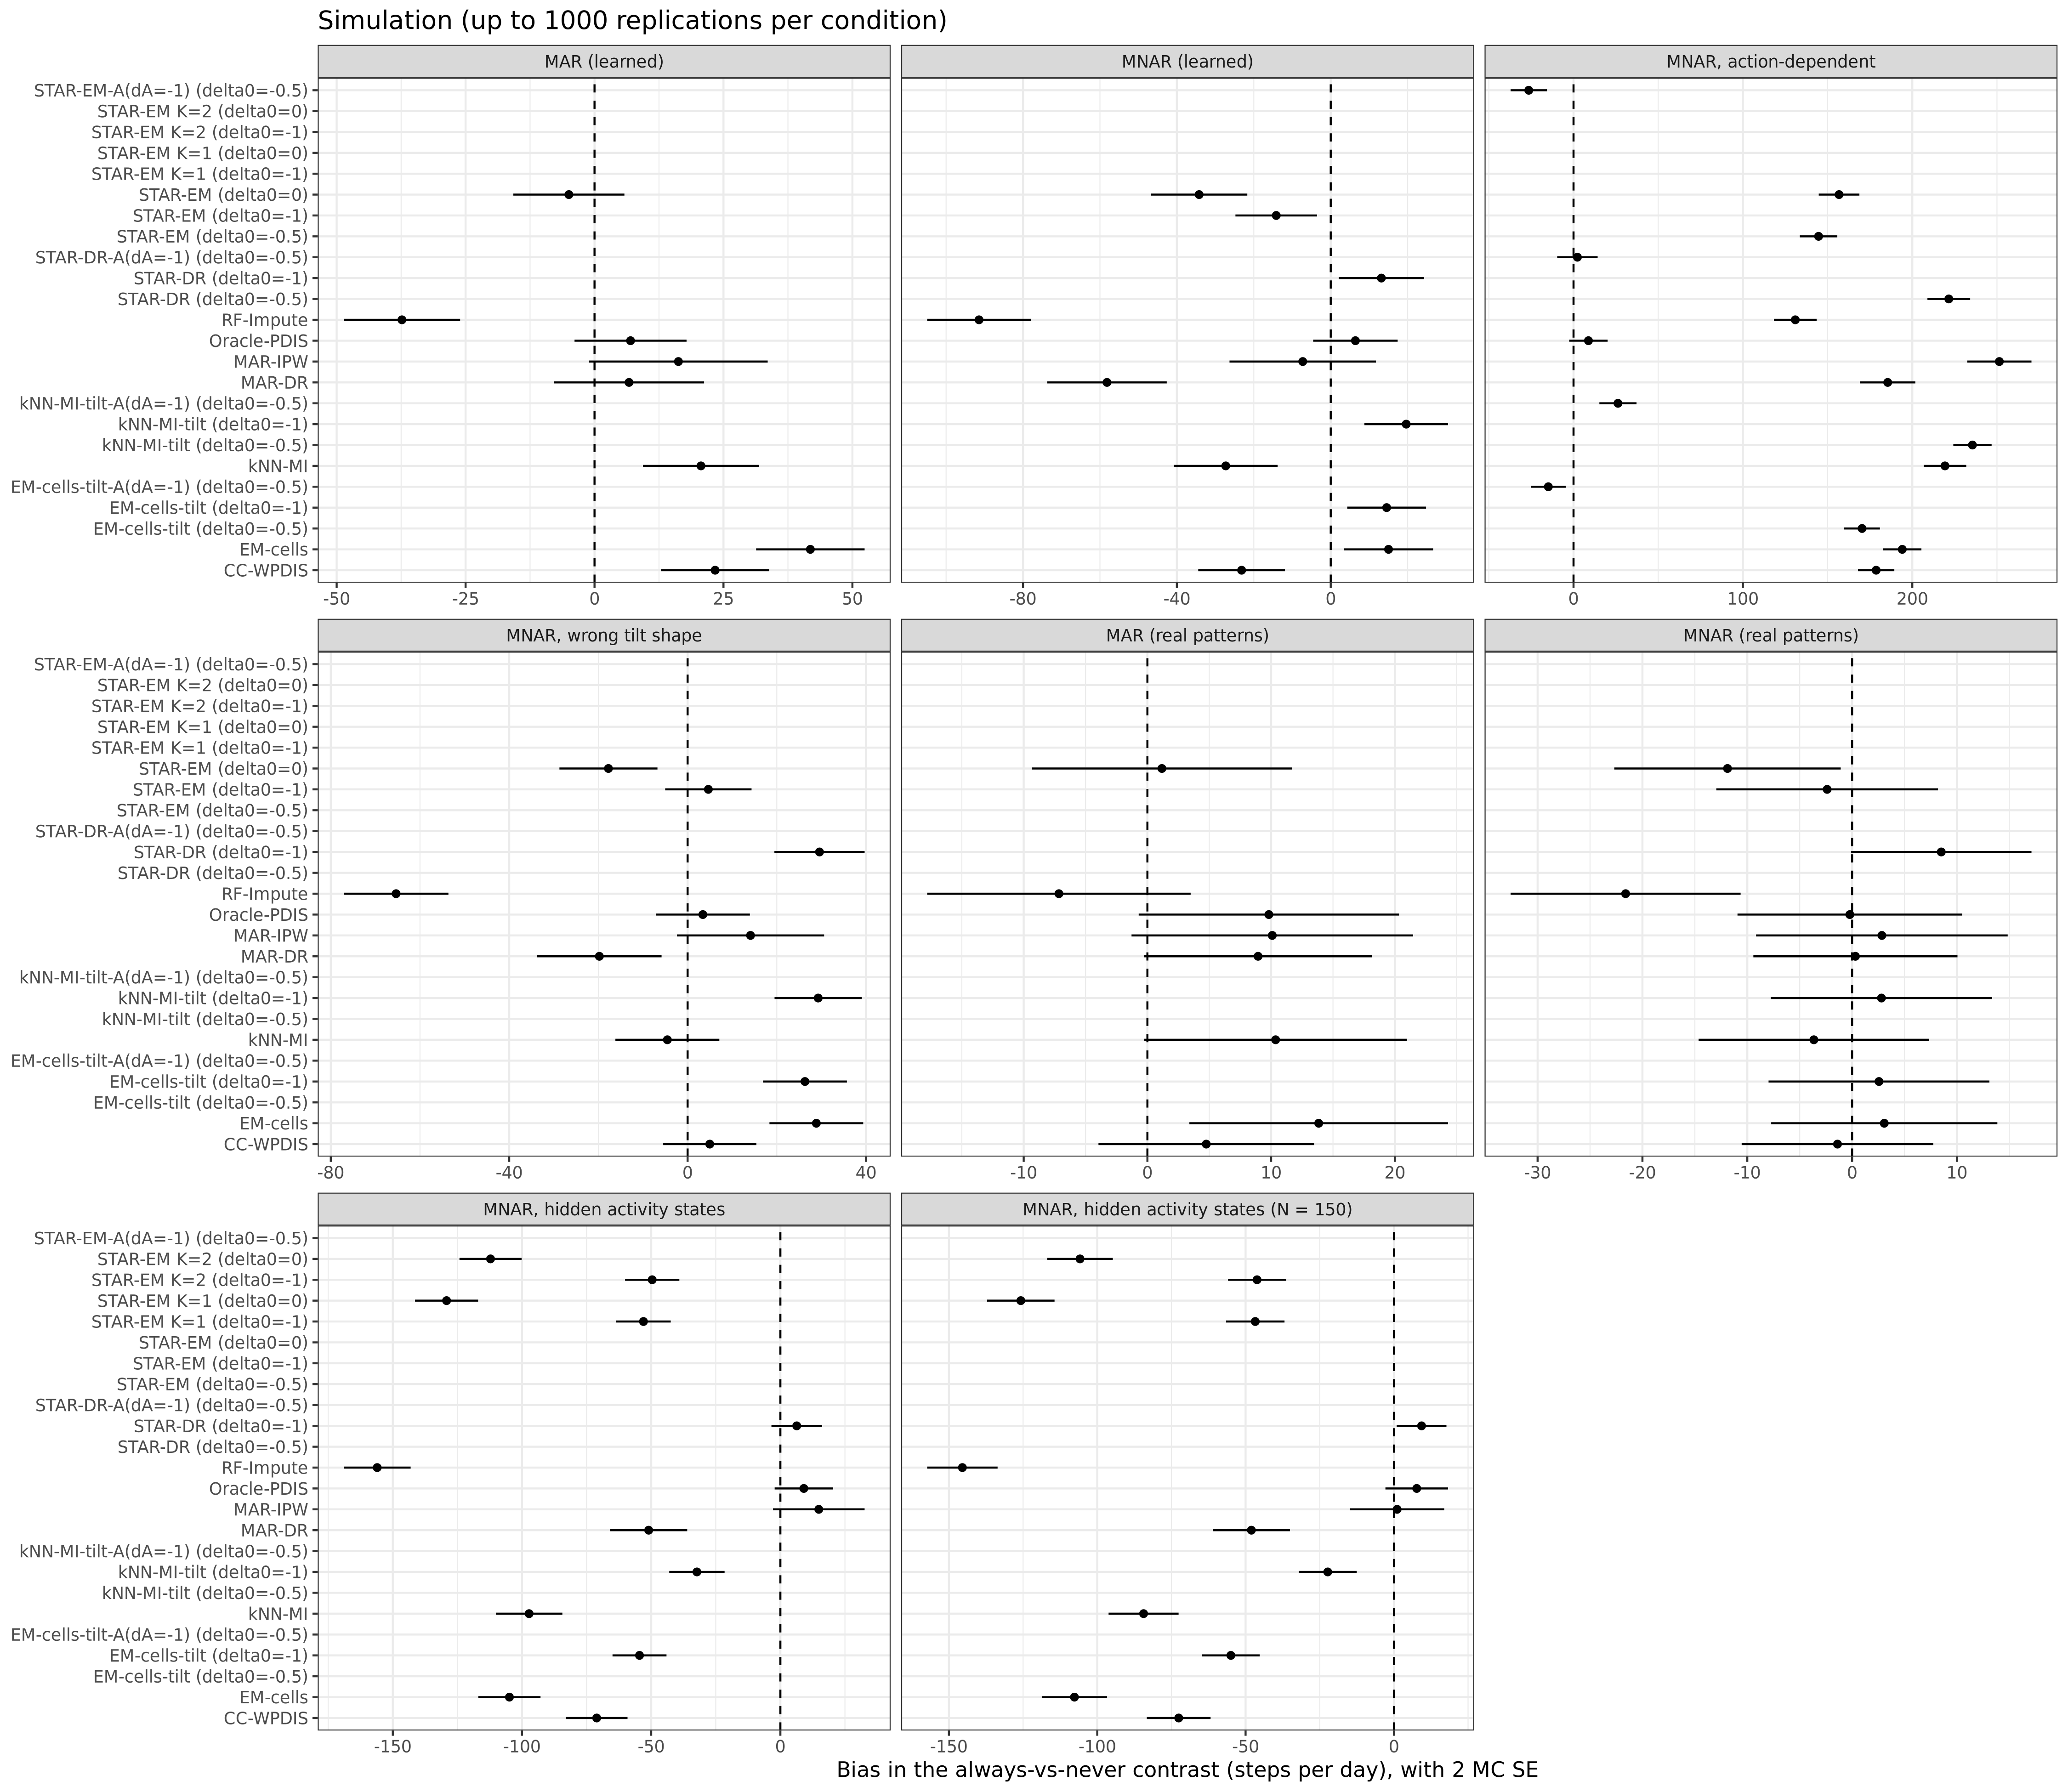
\includegraphics[width=0.97\textwidth]{fig_sim_bias.png}\caption{Bias in the always $-$ never contrast with $\pm$2 Monte Carlo SE, for every estimator and assumed tilt ($\delta_0$), by scenario. Rows are blank where an estimator was not run in that scenario.}\end{figure}

\begin{figure}[!htbp]
\centering
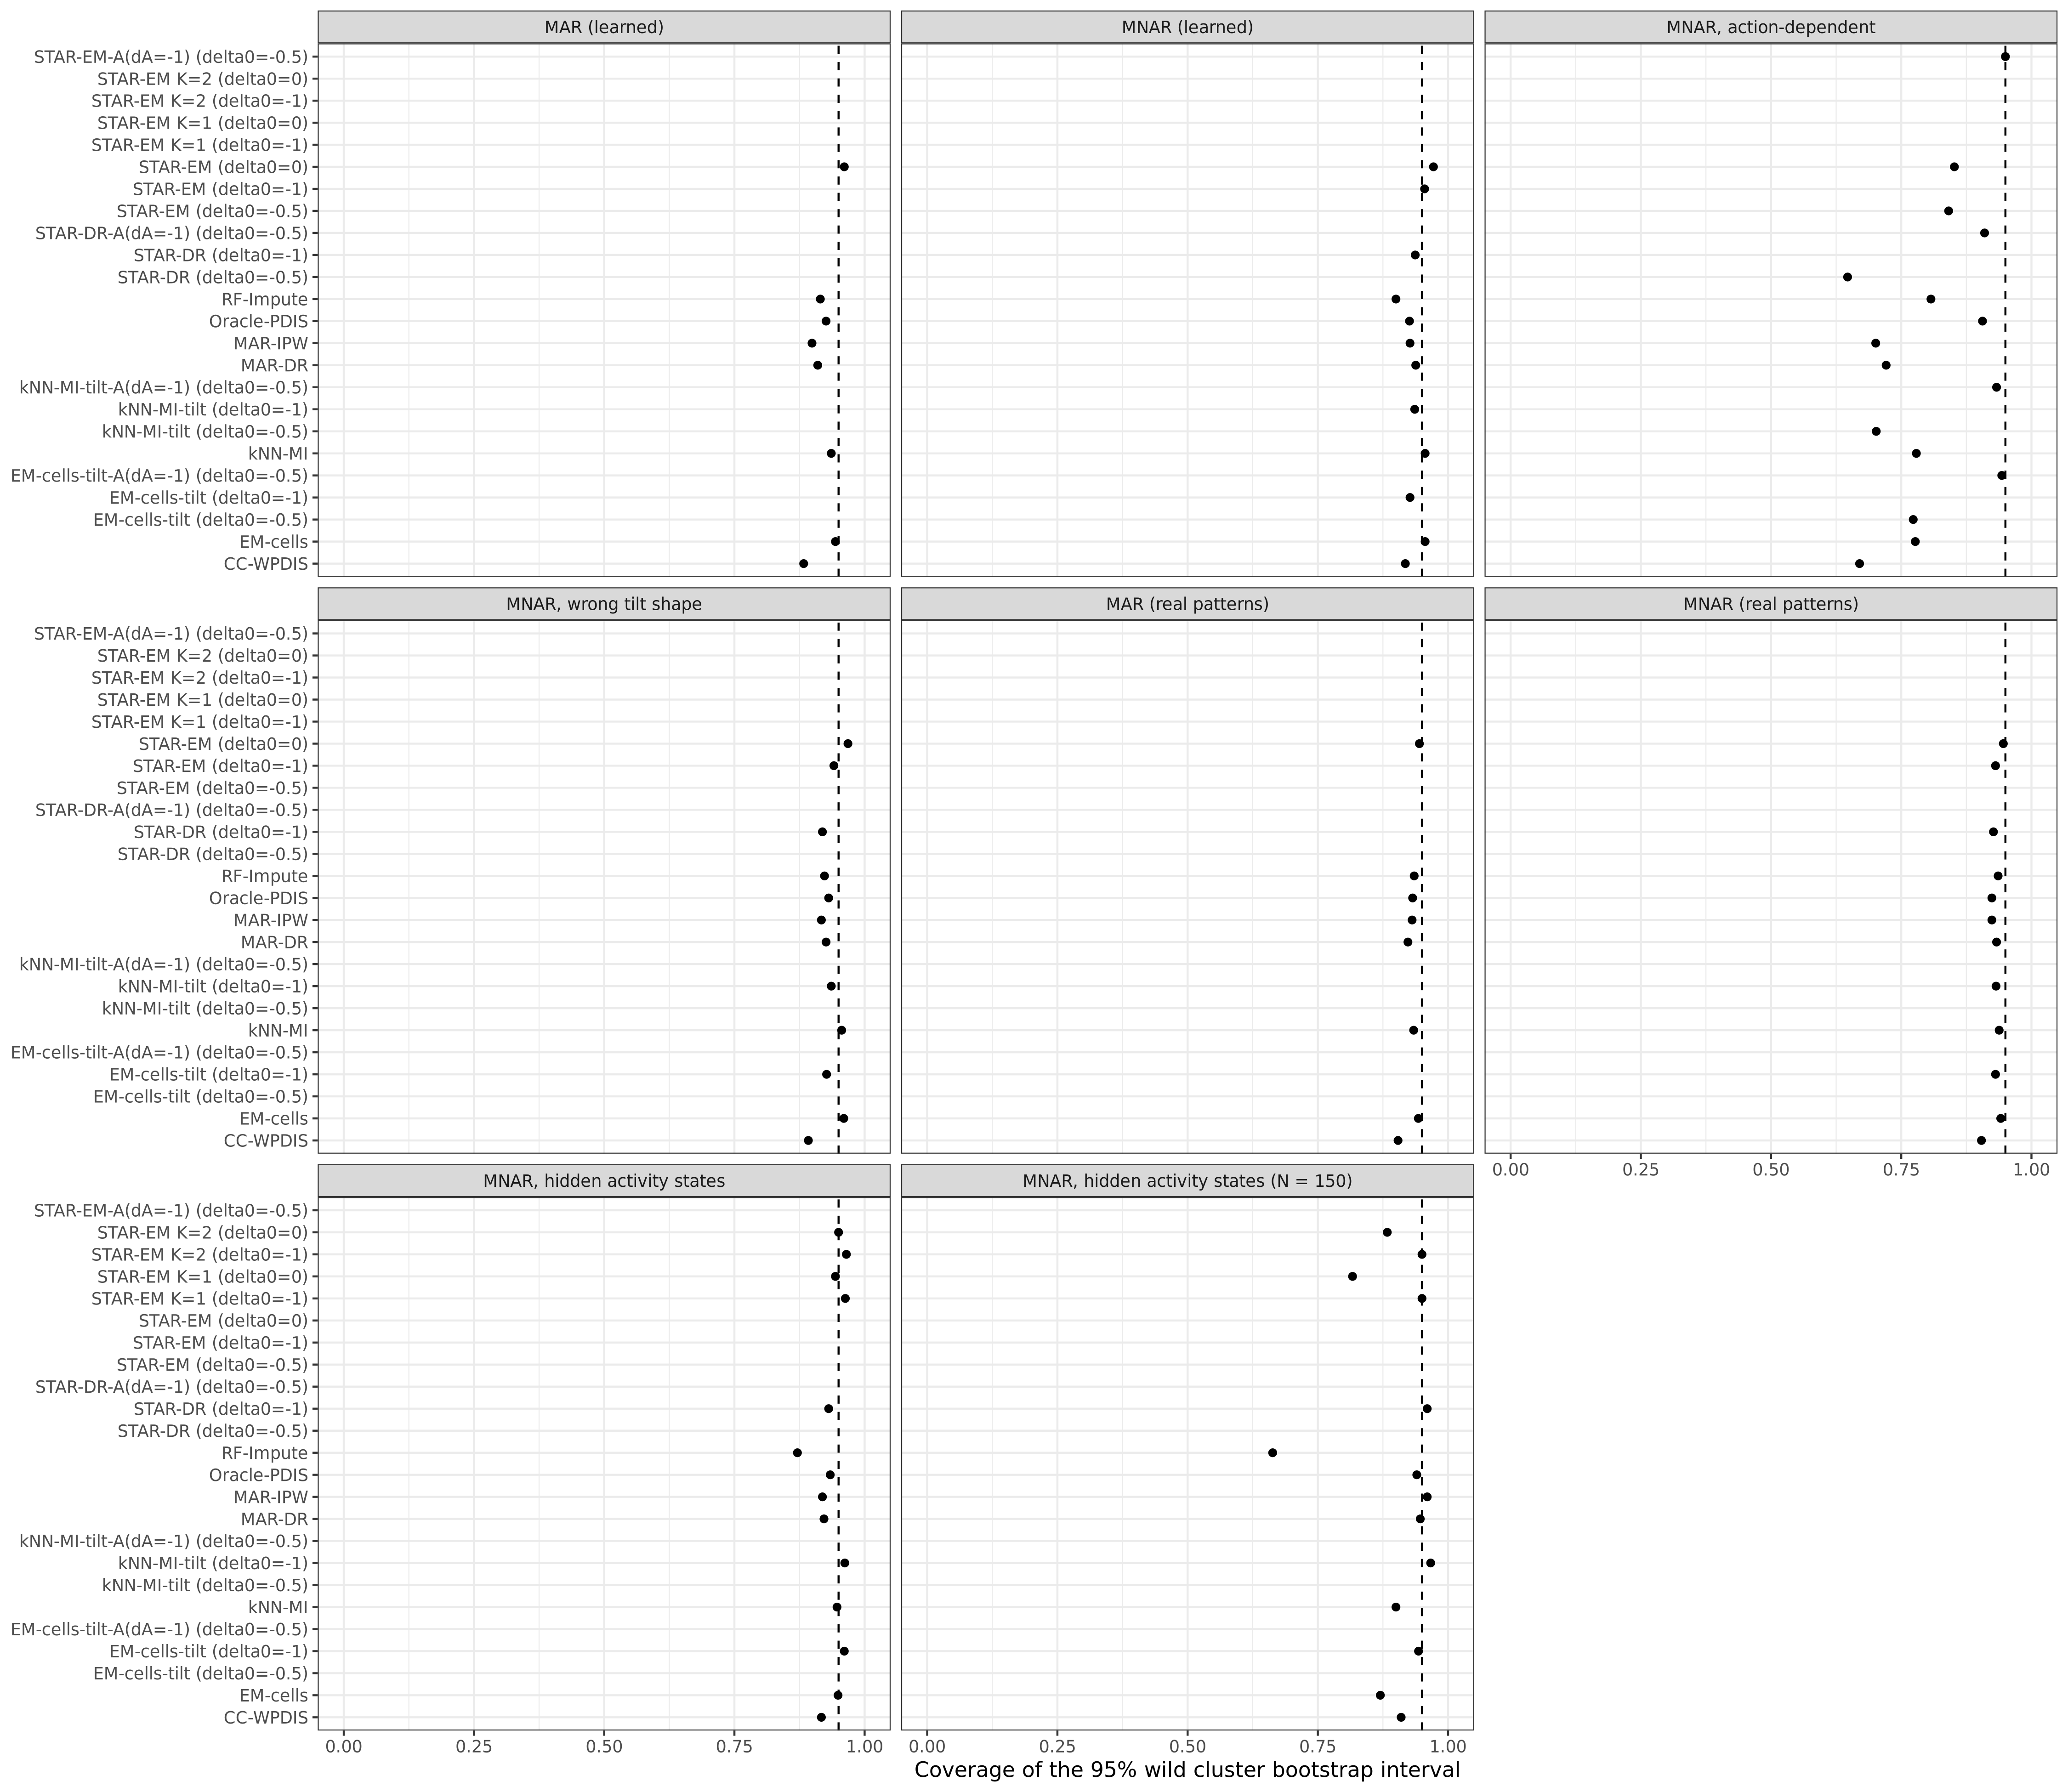
\includegraphics[width=0.97\textwidth]{fig4_sim_coverage.png}
\caption{Coverage of the 95\% wild cluster bootstrap interval for the always $-$ never contrast, for every estimator and assumed tilt ($\delta_0$), by scenario. The dashed line marks nominal 95\% coverage. Rows are blank where an estimator was not run in that scenario.}
\label{fig:coverage}
\end{figure}

\textbf{Precision.} Bias is only part of the picture. Table 4 compares the empirical SE, root mean squared error (RMSE) and average interval width of the oracle and the three doubly robust or joint-model estimators. Where it is unbiased, STAR-EM is about as precise as the complete-data oracle, because it analyses completed data with the same PDIS estimator. MAR-DR is less precise than the oracle in the learned-missingness scenarios, because its pseudo-rewards inflate observed rewards by inverse probabilities. With real missing patterns and with hidden states, STAR-DR is more precise than the oracle; the fitted-Q value model removes variance that importance sampling alone cannot.

\begin{table}[!htbp]\centering\footnotesize
\caption{Precision for the always $-$ never contrast: empirical SE / RMSE / mean width of the 95\% interval, in steps per day.}
\begin{tabular}{llrrrr}
\toprule
\textbf{\#} & \textbf{Scenario} & \textbf{Oracle} & \textbf{MAR-DR} & \textbf{STAR-EM} & \textbf{STAR-DR} \\
\midrule
1 & MAR with spells & 172 / 172 / 636 & 230 / 230 / 727 & 170 / 170 / 700 & 230 / 230 / 727 \\
2 & MNAR & 174 / 174 / 641 & 246 / 252 / 845 & 168 / 168 / 675 & 175 / 176 / 637 \\
3 & MNAR, action-dependent & 179 / 179 / 634 & 258 / 318 / 798 & 169 / 171 / 671 & 189 / 189 / 635 \\
4 & MNAR, wrong tilt shape & 167 / 167 / 636 & 221 / 221 / 749 & 153 / 153 / 628 & 160 / 163 / 574 \\
5 & MAR, real patterns & 166 / 167 / 637 & 145 / 146 / 542 & 166 / 166 / 659 & 145 / 146 / 542 \\
6 & MNAR, real patterns & 169 / 169 / 642 & 154 / 154 / 555 & 167 / 167 / 640 & 136 / 136 / 501 \\
7 & Hidden states, N = 37 & 178 / 179 / 683 & 236 / 241 / 823 & 167 / 175 / 670 & 155 / 155 / 584 \\
8 & Hidden states, N = 150 & 91 / 92 / 359 & 113 / 122 / 442 & 85 / 97 / 348 & 73 / 73 / 306 \\
\bottomrule
\end{tabular}
\end{table}

Estimators as in Table 3. The oracle here is PDIS on the complete rewards, not the best possible estimator; a doubly robust estimator on complete data would likely be more precise.

\textbf{Worst-case bounds.} The 95\% confidence region for the bounds contained the true value in at least 99.7\% of replications for every policy and contrast. The estimated bounds themselves can miss slightly in finite samples: for single policy values their point coverage fell as low as 72\%. They are also very wide. For the always $-$ never contrast their average width was 7,200 to 8,300 steps per day under learned and hidden-state missingness and about 2,200 with real patterns, against intervals of 500 to 850 for the tilted estimators. They are a useful reference, not a usable answer.

\textbf{Ignoring MNAR misleads.} Under reward-dependent MNAR (scenario 2), MAR-DR was off by $-$58 steps and random-forest imputation by $-$91. When missingness also depended on the prompt (scenario 3), every estimator without the action term was biased by +130 to +250 and coverage fell to 0.65--0.84. That included STAR-EM (+145) and STAR-DR (+222) when they left out $\delta_A$. With real missing patterns (scenarios 5 and 6) all methods did well, probably because the transplanted patterns are only weakly linked to the rewards.

\textbf{Both estimators work when $\delta$ is right.} With the correct tilt, STAR-EM and STAR-DR were within 30 steps of the truth in scenarios 1--6. STAR-EM's coverage stayed between 0.93 and 0.96 throughout (Figure~\ref{fig:coverage}), and it handled a tilt of the wrong shape better (+5 against +30).

\textbf{Hidden activity states favour STAR-DR.} In scenarios 7 and 8, STAR-DR was close to unbiased (+6 and +9) and at N = 150 had the smallest SE of any correction (73, against 85 for STAR-EM). STAR-EM kept a bias of about $-$50 that did not shrink with four times as many participants, so it comes from the model rather than the sample size. Without a tilt, STAR-EM's bias was $-$126 and its coverage fell to 0.82 at N = 150; random-forest imputation fell to 0.66.

\textbf{The hidden-state extension did not help.} STAR-EM with $K=2$ had the same bias as $K=1$ ($-$50 against $-$53 at N = 37; $-$46 against $-$47 at N = 150). Under the $\delta$ = $-$1 tilt its EM reached the 20-iteration cap in 99--100\% of fits; without a tilt over 99\% converged. The two-state model seems unable to separate a hidden cause of missingness from an assumed tilt that pushes in the same direction.

\begin{table}[!htbp]\centering\small
\caption{STAR-EM convergence in the hidden-state scenarios: percentage of fits that met the stopping rule within 20 iterations (mean iterations).}
\begin{tabular}{llrr}
\toprule
\textbf{Scenario} & \textbf{Tilt $\delta$} & \textbf{$K=1$} & \textbf{$K=2$} \\
\midrule
7 (N = 37) & 0 & 100\% (5.1) & 99.4\% (8.7) \\
7 (N = 37) & $-$1 & 90.7\% (18.0) & 1.3\% (20.0) \\
8 (N = 150) & 0 & 100\% (5.0) & 100\% (8.1) \\
8 (N = 150) & $-$1 & 98.7\% (18.1) & 0\% (20.0) \\
\bottomrule
\end{tabular}
\end{table}

In scenarios 1--6, where only $K=1$ was fitted, 96.3\% to 100\% of fits converged at every tilt. Non-convergence here means the stopping rule was not met, not that the fit diverged: the imputed means still moved by more than 1\% between iterations. Even so, a model that does not settle cannot be recommended without more work.

\textbf{Computing cost.} Per tilt, STAR-DR took about 17 seconds and 0.4 GB of memory. STAR-EM with five bootstrap EM refits took 136 seconds and 2.5 GB with $K=1$, and 874 seconds and 3.9 GB with $K=2$. For the EM-cells model, whose likelihood has a closed form, EM reached the same maximum as direct BFGS optimization in 4--6 iterations and 0.02--0.06 seconds, against 157--178 iterations and 1.5--2.1 seconds for BFGS on the HeartSteps data.

\section{Application to HeartSteps}

In HeartSteps, no policy contrast differed from zero under MAR, and none did anywhere on the tilt grid, so there is no tipping point to report: the data cannot tell these four policies apart, with or without MNAR.

\textbf{Data.} HeartSteps V1 (Klasnja et al., 2019) has 37 participants, 1,588 participant-days and 7,884 decisions. Participants were available at 80.3\% of decisions, and a suggestion was sent at 59.3\% of available decisions. Of the rewards, 9.4\% are missing. Observed rewards are zero 30.7\% of the time and heavily skewed (median 93 steps, mean 277, skewness 3.8). Mean steps were 248 after a suggestion, 235 when available but not sent, and 416 when unavailable, often because the person was already active.

\begin{table}[!htbp]\centering\small
\caption{HeartSteps V1: data used in the analysis.}
\begin{tabular}{p{0.55\textwidth}l}
\toprule
\textbf{Quantity} & \textbf{Value} \\
\midrule
Participants & 37 \\
Participant-days (episodes) & 1,588 \\
Decisions & 7,884 \\
Available for a suggestion & 80.3\% of decisions \\
Suggestion sent when available & 59.3\% (design: 60\%) \\
Rewards missing & 9.4\% \\
P(missing $|$ previous missing) & 66.8\% \\
P(missing $|$ previous observed) & 3.7\% \\
Zero steps among observed rewards & 30.7\% \\
Observed steps: median / mean / skewness & 93 / 277 / 3.8 \\
Mean (median) steps after a suggestion & 248 (78), n = 3,405 \\
Mean (median) steps, available but not sent & 235 (68), n = 2,341 \\
Mean (median) steps, unavailable & 416 (200), n = 1,399 \\
\bottomrule
\end{tabular}
\end{table}

The missingness is strongly persistent. A missing reward is followed by another missing reward 18 times as often as an observed one is, and missing rates vary widely across people (SD of person-level rates 0.12). This is the pattern that non-wear produces, and it is why STAR models missingness as spells rather than as independent events.

\textbf{Choice of K and EM diagnostics.} Held-out log-likelihood chose $K=1$ ($-$17,149, against $-$17,580 for $K=2$ and $-$17,550 for $K=3$, which did not converge in 20 iterations). The data show no hidden activity states that improve prediction, so in HeartSteps STAR-EM reduces to a spell-aware selection model. It converged at every point of the tilt grid, in 5 to 17 iterations. The EM-cells likelihood was identical ($-$17,541.003) at every $\delta$, which confirms that the data carry no information about $\delta$.

\textbf{What $\delta$ means in steps.} A tilt parameter is easier to judge when it is translated into the quantity people care about. Under MAR ($\delta$ = 0), STAR-EM imputes missing 30-minute windows with an average of 190 steps, somewhat below the observed mean of 277 because missingness is more common in contexts where people walk less. At $\delta_0$ = $-$0.5 the imputed mean falls to 91 steps, at $\delta_0$ = $-$1 to 36, and at $\delta_0$ = $-$1.5 to 13, close to the floor of no movement at all. In the other direction, $\delta_0$ = 1 implies 452 steps and $\delta_0$ = 1.5 implies 555. The grid from $-$1.5 to 1.5 therefore runs from ``the tracker was off because the person was sitting still'' to ``the tracker was off because the person was out exercising without it'', which spans every story we consider plausible. Adding $\delta_A$ = $-$0.5 lowers the imputed mean further on decisions where a suggestion was sent (for example, 28 rather than 36 steps at $\delta_0$ = $-$1).

\textbf{Estimates under MAR.} Table 7 shows the three contrasts at $\delta$ = 0. Every 95\% interval includes zero. The doubly robust estimate of always $-$ never (+140) has the opposite sign to the imputation estimates ($-$119 to $-$161). The gap comes from the never policy (1,309 steps by MAR-DR against about 1,500 by the imputation methods); this value rests only on decisions where no prompt was sent, each weighted by 1/0.4. The intervals overlap heavily, so the disagreement is within the noise of 37 participants.

\begin{table}[!htbp]\centering\small
\caption{HeartSteps policy contrasts under MAR ($\delta$ = 0), in steps per day: estimate [95\% wild cluster bootstrap interval].}
\begin{tabular}{llrr}
\toprule
\textbf{Method} & \textbf{Always $-$ never} & \textbf{Tailored $-$ always} & \textbf{Capped $-$ always} \\
\midrule
Complete case & +72 [$-$171, 333] & $-$137 [$-$285, 23] & $-$44 [$-$212, 143] \\
MAR-IPW & $-$119 [$-$557, 292] & $-$125 [$-$379, 145] & $-$28 [$-$268, 230] \\
RF imputation & $-$156 [$-$540, 208] & $-$57 [$-$242, 139] & +33 [$-$190, 259] \\
kNN multiple imputation & $-$157 [$-$549, 229] & $-$59 [$-$273, 157] & +39 [$-$196, 279] \\
EM-cells & $-$133 [$-$527, 263] & $-$72 [$-$291, 151] & +30 [$-$196, 253] \\
STAR-EM ($K=1$) & $-$161 [$-$597, 241] & $-$57 [$-$276, 174] & +35 [$-$189, 259] \\
MAR-DR & +140 [$-$220, 470] & $-$161 [$-$392, 66] & $-$139 [$-$331, 63] \\
Worst-case bounds & [$-$1,325, 940] & [$-$1,126, 1,108] & [$-$1,009, 999] \\
\bottomrule
\end{tabular}
\end{table}

\textbf{Policy values and bounds.} Table 8 shows the value of each policy, not just the contrasts. Every method puts each policy at roughly 1,300 to 1,500 steps per day, and the worst-case bounds run from about 1,200 to 2,600. The bounds are lopsided: missing rewards can only add steps, so the upper bound sits far above every estimate, while the lower bound sits close to them. Two estimates of the never policy fall slightly below its lower bound: complete case (1,362) and MAR-DR (1,309), against a bound of 1,375. This is possible because the bounds use plain importance sampling, while complete case uses self-normalized weights and MAR-DR leans on a fitted value model. The gap is well inside the sampling error (the MAR-DR interval is 953 to 1,679), but it is a warning sign. The never policy is estimated only from decisions where no suggestion was sent, so its value model has the least data behind it, and this is also the policy on which MAR-DR and the imputation methods disagree.

\begin{table}[!htbp]\centering\footnotesize
\caption{HeartSteps policy values under MAR, in steps per day: estimate [95\% interval], with worst-case bounds.}
\begin{tabular}{llrrr}
\toprule
\textbf{Policy} & \textbf{Complete case} & \textbf{MAR-DR} & \textbf{STAR-EM ($K=1$)} & \textbf{Worst-case bounds} \\
\midrule
Always & 1,435 [1,220, 1,657] & 1,449 [1,209, 1,682] & 1,343 [1,119, 1,561] & [1,259, 2,315] \\
Never & 1,362 [1,086, 1,656] & 1,309 [953, 1,679] & 1,503 [1,084, 1,961] & [1,375, 2,585] \\
Tailored & 1,298 [1,027, 1,560] & 1,288 [1,014, 1,566] & 1,286 [991, 1,590] & [1,189, 2,367] \\
Capped & 1,391 [1,155, 1,626] & 1,311 [1,082, 1,527] & 1,377 [1,105, 1,652] & [1,306, 2,258] \\
\bottomrule
\end{tabular}
\end{table}

\textbf{Sensitivity to MNAR.} STAR-DR and STAR-EM were run over $\delta_0$ from $-$1.5 to 1.5 in steps of 0.25, with $\delta_A$ = 0 and $-$0.5. Across that grid the STAR-DR estimate of always $-$ never moved from +51 to +357 steps per day, rising as missing rewards were assumed to be higher than observed ones; the STAR-EM estimate stayed between $-$116 and $-$218. No interval excluded zero for any contrast. The worst-case bounds span about 2,000 steps per day for each contrast, so without some assumption about the missingness the data cannot rule out large effects in either direction.

The two estimators respond to the tilt very differently. STAR-EM's imputed rewards move a great deal across the grid (from 13 to 555 steps per window), yet its contrasts barely change, because the shift applies to missing rewards under every policy alike and largely cancels in a difference. STAR-DR's contrasts move more, probably because its pseudo-rewards also reweight the observed rewards, and that reweighting differs between decisions with and without a suggestion. With only 9.4\% of rewards missing, neither curve gets close to changing a conclusion, but the difference in behaviour is worth knowing before applying the framework to a trial with more missing data.

\begin{figure}[!htbp]\centering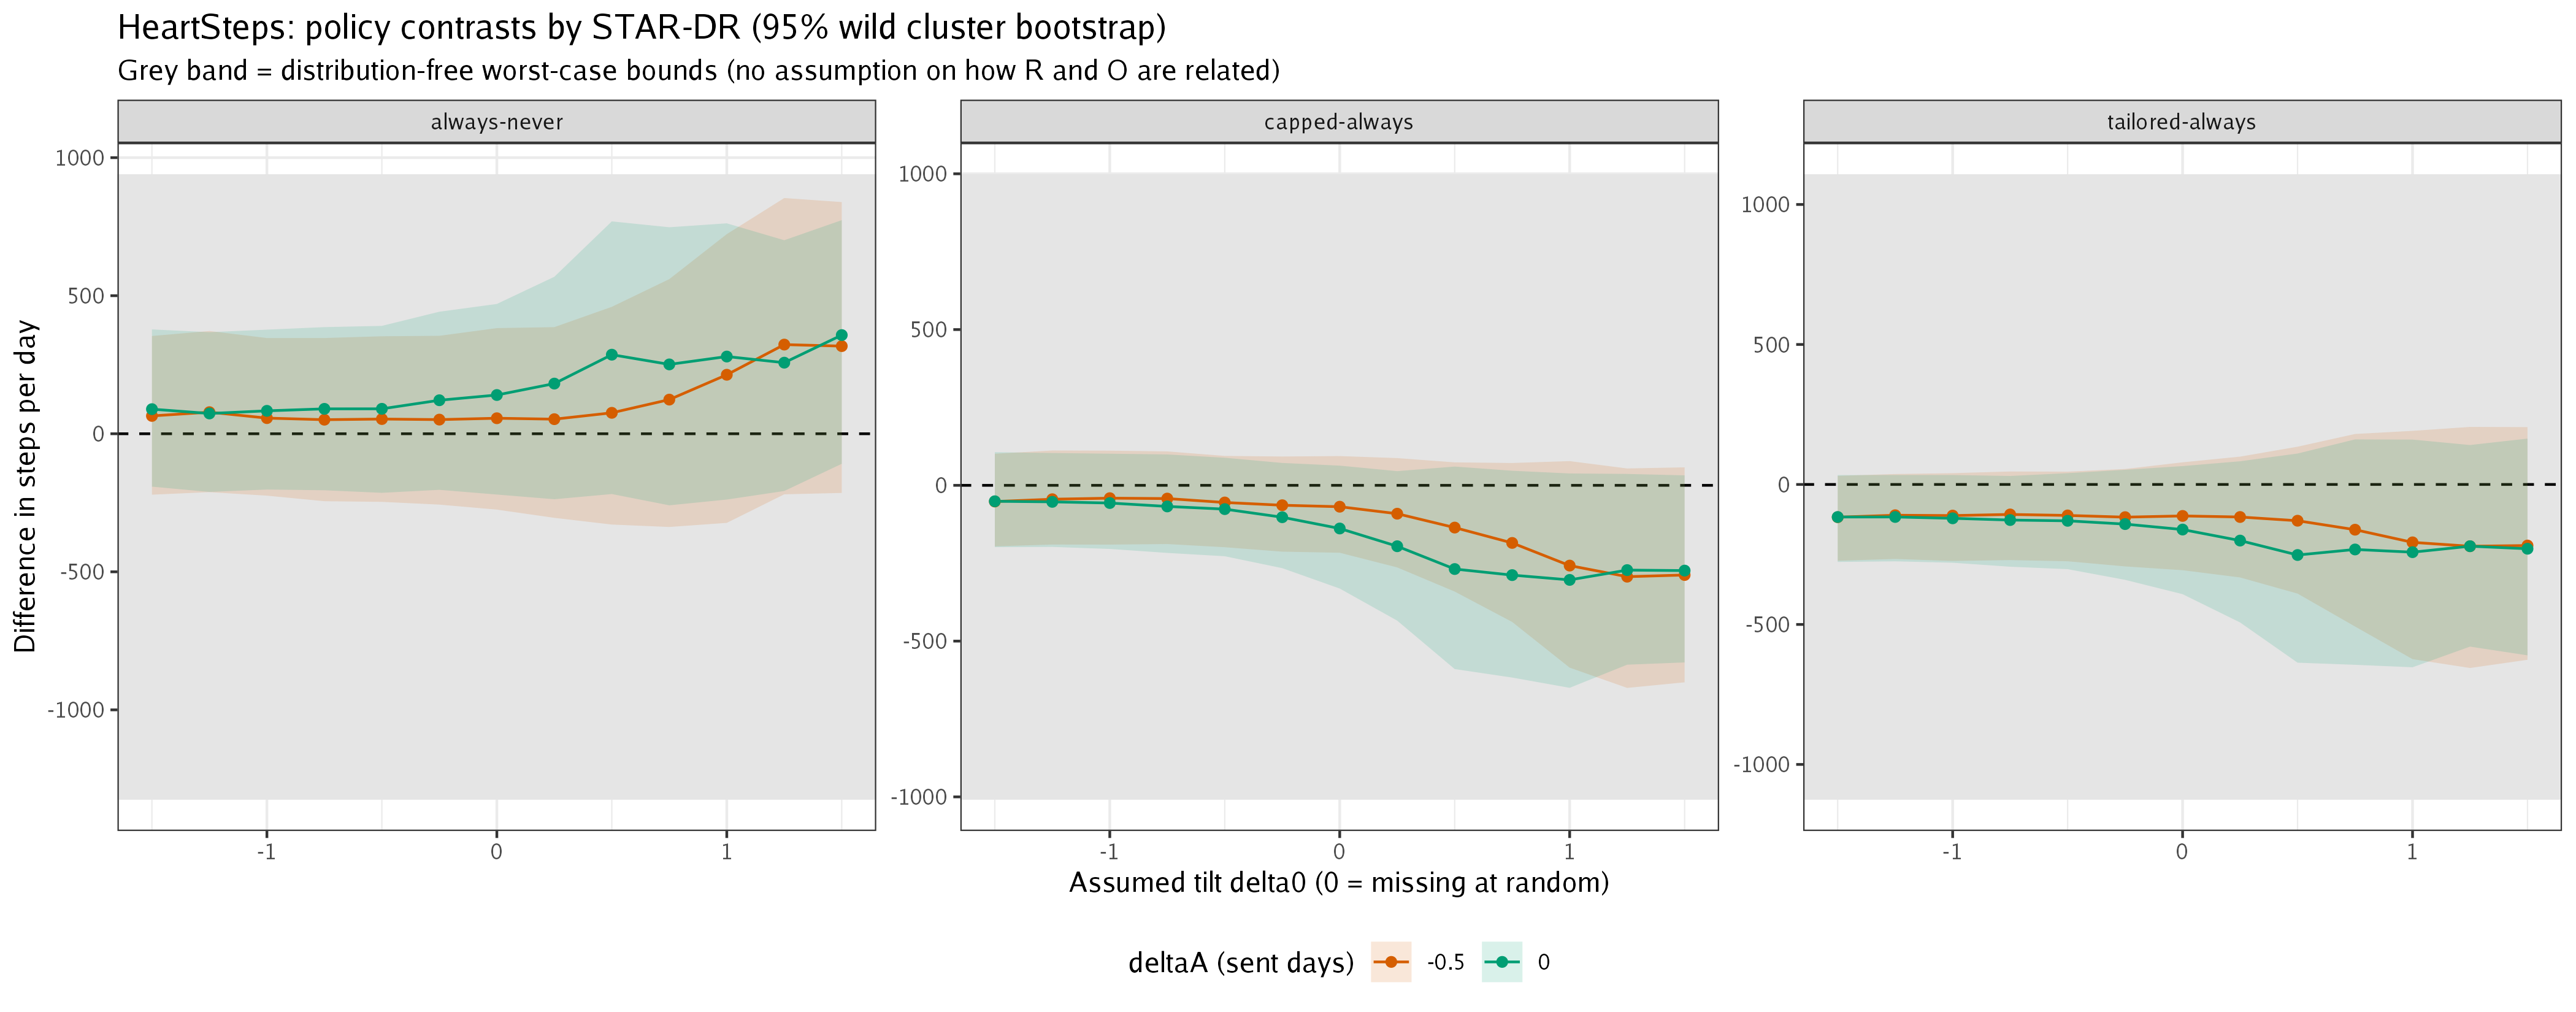
\includegraphics[width=0.97\textwidth]{fig_heartsteps_tipping.png}\caption{STAR-DR estimates of the three HeartSteps contrasts as the assumed tilt $\delta_0$ varies, for $\delta_A$ = 0 (green) and $\delta_A$ = $-$0.5 (orange), with 95\% wild cluster bootstrap bands. The grey band shows the worst-case bounds, which assume nothing about the missingness.}\end{figure}

\textbf{Computing cost.} On the real data, one tilt took 838 seconds for STAR-EM with five bootstrap EM refits and 114 seconds for STAR-DR.

\section{Discussion}

When wearable rewards may be missing not at random, the question an analyst can answer is not ``what is the policy value?'' but ``how much MNAR would it take to change my conclusion?'' STAR answers that question for OPE in MRTs, and the simulations give a clear recommendation: use STAR-DR as the primary estimator and report STAR-EM beside it.

\textbf{Recommendations for practice.}

\begin{enumerate}

\item \textbf{Always include an action term in the sensitivity analysis.} When missingness depends on whether a prompt was sent, every estimator without $\delta_A$ was badly biased, including both STAR estimators. Since a prompt can plausibly remind someone to wear the device, $\delta_A$ should be varied alongside $\delta_0$.

\item \textbf{Prefer STAR-DR as the default.} It was close to unbiased in every scenario when given the right tilt, it was the only method robust to hidden activity states, and it was about seven to eight times cheaper than STAR-EM.

\item \textbf{Use STAR-EM as a check.} Its coverage stayed close to 95\% throughout and it was less sensitive to a tilt of the wrong shape. When the two estimators agree, the conclusion does not depend on the modelling route. When they disagree, as for always $-$ never in HeartSteps, the disagreement is itself a finding.

\item \textbf{Report worst-case bounds.} They show how much of any conclusion rests on the sensitivity assumption.

\end{enumerate}

\textbf{What the EM work shows.} For a model with a closed-form likelihood, EM reached the same maximum as direct optimization 25 to 100 times faster. For the full joint model, EM is the only practical fitting route, because forests have no gradient. But the hidden-state layer did not pay for itself: it was not selected in HeartSteps, it gave no gain in simulation, and it failed to converge under a nonzero tilt. The joint-model idea may still be worth pursuing, but with better starting values, a longer iteration budget, or a parametric M-step for the transition model.

\textbf{Why the joint model struggles with hidden states.} In scenarios 7 and 8 the missingness comes from a hidden low-activity state, and no tilt is true. STAR-EM with $K=1$ can only express that dependence through the tilt and through the observed history, so with $\delta$ = $-$1 it captures part of the effect and leaves a bias of about $-$50 steps. In principle $K=2$ should capture the rest, but in practice it did not. Two features of the setting work against it. First, the hidden state and the tilt explain the same pattern, low rewards that tend to be missing, so when both are present the likelihood has a ridge along which state probabilities and tilt trade off. That would explain why $K=2$ converged at $\delta$ = 0 but almost never at $\delta$ = $-$1. Second, the forests in the M-step are refitted at each iteration and add noise that can swamp the small likelihood gains that separate a two-state model from a one-state model. STAR-DR avoids both problems. It never tries to recover the hidden state; it only needs the tilted mean of the missing rewards given the history, and its fitted-Q step absorbs much of the remaining structure. This is an argument for doubly robust estimation when the source of MNAR is unknown, not an argument against joint modelling in general. A joint model with a parametric emission layer and a more careful M-step may well do better than ours.

\textbf{Choosing a plausible range for $\delta$.} The tilt is only useful if analysts can say which values are believable. Translating $\delta$ into imputed steps, as in Section 6, is the most direct way: a reader who thinks people rarely remove their trackers to go running can rule out large positive values, and one who thinks non-wear is mostly sleep or desk work can focus on values below zero. External data can narrow the range further. Wear-time studies that record when devices are on but not counting steps, or trials with a second sensor such as a phone accelerometer, can estimate how active people are during non-wear. Expert judgement can also be elicited directly as a statement about steps, then converted into $\delta$. We recommend reporting the full grid regardless, because a reader's plausible range may differ from the analyst's.

\textbf{Relation to shadow-variable methods.} STAR and the shadow-variable estimators of Wang et al. (2025) and Wei et al. (2026) answer different questions. A shadow-variable method gives one estimate that is correct if its identifying condition holds; STAR gives a curve of estimates, each correct if the assumed tilt holds. The two can be combined. If a credible shadow variable exists, its estimate is one point on the STAR curve, and the curve shows how much the conclusion depends on that point. If no credible shadow variable exists, as is common when non-wear removes the reward and the next state together, the curve is the honest answer.

\textbf{Relation to excursion-effect analyses.} The usual primary analysis of an MRT estimates causal excursion effects: the average effect of a prompt at a decision point, compared with no prompt, often moderated by context (Boruvka et al., 2018). Missing rewards bias those analyses in the same way, and the tilt applies to them directly, since an excursion effect is a contrast of mean rewards at one decision. The policy values studied here add something excursion effects cannot give. They account for how a prompt now changes availability, behaviour and the chance of later prompts, and they compare rules a designer could actually deploy. The always $-$ never contrast is the policy-level counterpart of the overall excursion effect. In HeartSteps its interval spans several hundred steps per day in both directions under every assumption we considered, so the short-term effect of suggestions on steps in the following 30 minutes reported by Klasnja et al. (2019) does not, on this evidence, translate into a detectable difference in total daily steps.

\textbf{Implications for trial design.} The analysis also points to cheap changes in how MRTs are run. Recording device wear time, not only step counts, would separate ``zero steps'' from ``not worn'' and make the missingness indicator more accurate. A short prompt asking why a tracker was off, sent after a long gap, would give direct evidence about $\delta$. Finally, the HeartSteps sample of 37 people was too small to distinguish these policies under any assumption about missingness; precision, more than bias, limited the conclusions here.

\textbf{Limitations.} This is one trial with one wearable outcome and 37 participants, so the HeartSteps intervals are wide and the application is mainly an illustration. The simulations used a 30\% missing rate, about three times the real rate, and the learned generator produced shorter spells than the real data. The linear-in-q tilt is one way to express MNAR; scenario 4 tests one alternative, and there are others. Finally, the framework relies on a known behaviour policy, so it applies to randomized trials, not to observational mobile health data.

\textbf{Future work.} Natural next steps are a formal proof of the double robustness of the tilted pseudo-reward, guidance for choosing a plausible range of $\delta$ from external data such as wear-time studies, and an application to a larger MRT with more participants and a higher missing rate.

\section{Conclusion}

Wearable outcomes in micro-randomized trials go missing in spells, and the reasons they go missing may be tied to the very behaviour the trial is trying to change. Because the data cannot reveal how strong that link is, evaluating a decision rule from such a trial should end with a sensitivity analysis, not a single number. STAR provides one. A single tilt parameter, allowed to differ on decisions with and without a prompt, expresses the departure from MAR, and two estimators carry it through to policy values: a joint model fitted by EM and a tilted doubly robust estimator. In a plasmode simulation built from HeartSteps, both removed most of the bias when the tilt was right, ignoring a prompt-dependent tilt was the costliest mistake, and the doubly robust estimator was the more reliable and much cheaper of the two. In HeartSteps itself the four notification policies could not be told apart under any assumption on the grid. That is a statement about the size of the trial more than about missing data, and the framework makes it possible to say so with confidence rather than by default.

\section*{References}
\begin{list}{}{\setlength{\leftmargin}{0.5in}\setlength{\itemindent}{-0.5in}\setlength{\itemsep}{3pt}}

\item Boruvka, A., Almirall, D., Witkiewitz, K., \& Murphy, S. A. (2018). Assessing time-varying causal effect moderation in mobile health. \textit{Journal of the American Statistical Association, 113}(523), 1112--1121.

\item Chernozhukov, V., Chetverikov, D., Demirer, M., Duflo, E., Hansen, C., Newey, W., \& Robins, J. (2018). Double/debiased machine learning for treatment and structural parameters. \textit{The Econometrics Journal, 21}(1), C1--C68.

\item Dempster, A. P., Laird, N. M., \& Rubin, D. B. (1977). Maximum likelihood from incomplete data via the EM algorithm. \textit{Journal of the Royal Statistical Society: Series B, 39}(1), 1--38.

\item Follmann, D., \& Wu, M. (1995). An approximate generalized linear model with random effects for informative missing data. \textit{Biometrics, 51}(1), 151--168.

\item Gassiat, É., Cleynen, A., \& Robin, S. (2016). Inference in finite state space non parametric hidden Markov models and applications. \textit{Statistics and Computing, 26}(1--2), 61--71.

\item Horowitz, J. L., \& Manski, C. F. (2000). Nonparametric analysis of randomized experiments with missing covariate and outcome data. \textit{Journal of the American Statistical Association, 95}(449), 77--84.

\item Jiang, N., \& Li, L. (2016). Doubly robust off-policy value evaluation for reinforcement learning. \textit{Proceedings of the 33rd International Conference on Machine Learning} (PMLR 48, pp. 652--661).

\item Klasnja, P., Smith, S., Seewald, N. J., Lee, A., Hall, K., Luers, B., Hekler, E. B., \& Murphy, S. A. (2019). Efficacy of contextually tailored suggestions for physical activity: A micro-randomized optimization trial of HeartSteps. \textit{Annals of Behavioral Medicine, 53}(6), 573--582.

\item Le, H., Voloshin, C., \& Yue, Y. (2019). Batch policy learning under constraints. \textit{Proceedings of the 36th International Conference on Machine Learning} (PMLR 97, pp. 3703--3712).

\item Morris, T. P., White, I. R., \& Crowther, M. J. (2019). Using simulation studies to evaluate statistical methods. \textit{Statistics in Medicine, 38}(11), 2074--2102.

\item Nahum-Shani, I., Smith, S. N., Spring, B. J., Collins, L. M., Witkiewitz, K., Tewari, A., \& Murphy, S. A. (2018). Just-in-time adaptive interventions (JITAIs) in mobile health: Key components and design principles for ongoing health behavior support. \textit{Annals of Behavioral Medicine, 52}(6), 446--462.

\item Precup, D., Sutton, R. S., \& Singh, S. (2000). Eligibility traces for off-policy policy evaluation. \textit{Proceedings of the 17th International Conference on Machine Learning} (pp. 759--766). Morgan Kaufmann.

\item Rubin, D. B. (1976). Inference and missing data. \textit{Biometrika, 63}(3), 581--592.

\item Scharfstein, D. O., Rotnitzky, A., \& Robins, J. M. (1999). Adjusting for nonignorable drop-out using semiparametric nonresponse models. \textit{Journal of the American Statistical Association, 94}(448), 1096--1120.

\item Wang, H., Xu, Y., Lu, W., \& Song, R. (2025). Off-policy evaluation under nonignorable missing data. \textit{Proceedings of the 42nd International Conference on Machine Learning} (PMLR 267).

\item Webb, M. D. (2023). Reworking wild bootstrap-based inference for clustered errors. \textit{Canadian Journal of Economics, 56}(3), 839--858.

\item Wei, Z., Qu, A., \& Miao, R. (2026). Off-policy evaluation for missingness-aware policies in MDPs with rewards missing not at random. \textit{Proceedings of the 43rd International Conference on Machine Learning} (PMLR 306).

\item Yu, J., \& Qian, T. (2024). Doubly robust estimation of causal excursion effects in micro-randomized trials with missing longitudinal outcomes. arXiv:2411.10620.

\item Zhang, S., Dziak, J. J., Benson, L., Yap, J. R. T., Jones, D. R., Lam, C. Y., Potter, L. N., Wetter, D. W., \& Nahum-Shani, I. (2025). Missing data in microrandomized trials: Challenges and opportunities. \textit{Behavior Research Methods, 57}(12), Article 344.

\end{list}

\appendix

\section{Computing details}

All analyses were written in R 4.4 using data.table, ranger (random and probability forests), rpart (the boosted missingness trees), FNN (nearest-neighbour imputation) and ggplot2. The code runs in four modes: preparation (data, true policy values and generator checks), the real-data analysis, one simulation task, and a combine step that builds every simulation table and figure from the finished tasks.

\textbf{Simulation runs.} Each scenario with 37 participants was split into 40 array tasks of 25 replications, and scenario 8 into 150 tasks of 2 replications, so a failed task could be rerun without repeating the others. Each task drew its seed from set.seed(100) and its task number, so results do not depend on which cluster ran a task. Scenarios 1--7 ran on the shared CPU partition of Anvil (Purdue University) through an ACCESS allocation, with one or two cores per task. The hidden-state scenarios were the most expensive: with STAR-EM fitted at $K=1$ and $K=2$, a scenario 7 task of 25 replications took 5 to 7 hours. When the Anvil allocation ran low, scenario 8 and two unfinished scenario 7 tasks were run on the Alpine cluster (University of Colorado Boulder) through RMACC, where a scenario 8 task of two replications took about 57 minutes. The combine step read all 430 task files and took under two minutes.

\textbf{Real-data run.} The HeartSteps analysis ran once on Anvil. It fitted every estimator at 26 tilt combinations (13 values of $\delta_0$ by 2 values of $\delta_A$), with intervals from the wild cluster bootstrap.

\begin{table}[H]\centering\small
\caption{Computing cost per tilt: mean seconds per simulated trial (N = 37) and seconds on the HeartSteps data.}
\begin{tabular}{p{0.38\textwidth}rp{0.17\textwidth}p{0.16\textwidth}}
\toprule
\textbf{Component} & \textbf{Simulation (s)} & \textbf{HeartSteps (s)} & \textbf{Memory (MB)} \\
\midrule
Nuisance forests shared by IPW, RF imputation and DR & 7.5 & 29.7 & 273 \\
STAR-DR: pseudo-rewards and fitted-Q evaluation & 16.8 & 113.6 & 258 \\
STAR-EM ($K=1$): EM fit and five bootstrap refits & 136.3 & 837.9 & 442 \\
STAR-EM ($K=2$): EM fit and five bootstrap refits & 874.2 & not run ($K=1$ chosen) & --- \\
EM-cells: fitting the selection model & 0.4 & 4.4 & 160 \\
kNN: drawing 20 imputations & 0.3 & 1.1 & 262 \\
Complete case, MAR-IPW or RF imputation estimate & 0.7 & 0.7 & 166 \\
\bottomrule
\end{tabular}
\end{table}

The real-data run took longer per tilt than one simulated trial. In both settings STAR-EM was the dominant cost, about seven to eight times STAR-DR with $K=1$.

\section{Reproducibility}

HeartSteps V1 is publicly available (Klasnja et al., 2019). The analysis code, the SLURM job scripts for both clusters, and every table in this paper are available from the author on request. All random numbers derive from set.seed(100).
\end{document}
